\documentclass{article}

\usepackage{amsmath}
\usepackage{color}
\usepackage{epigraph}
\usepackage{fourier}
\usepackage{fullpage}
\usepackage{fullpage}
\usepackage{graphicx}
\usepackage{listings}
\usepackage{url}
\usepackage{xspace}
\usepackage[colorlinks=true,urlcolor=blue]{hyperref}

\usepackage{fancyhdr}
\pagestyle{fancy}
\fancyhf{}

\fancypagestyle{plain}{%
  \fancyhf{}
  \renewcommand{\headrulewidth}{0pt}
  \renewcommand{\footrulewidth}{0pt}
  \lfoot{\textcopyright{} 2021 Darrell Long}
  \rfoot{\thepage}
}

\pagestyle{plain}

\definecolor{codegreen}{rgb}{0,0.5,0}
\definecolor{codegray}{rgb}{0.5,0.5,0.5}
\definecolor{codepurple}{rgb}{0.58,0,0.82}

\lstloadlanguages{C,make,python,fortran}

\lstdefinestyle{c99}{
    morekeywords={bool, uint8_t, uint16_t, uint32_t, uint64_t, int8_t, int16_t, int32_t, int64_t},
    commentstyle=\color{codegreen},
    keywordstyle=\color{magenta},
    numberstyle=\tiny\color{codegray},
    identifierstyle=\color{blue},
    stringstyle=\color{codepurple},
    basicstyle=\ttfamily,
    breakatwhitespace=false,
    breaklines=true,
    captionpos=b,
    keepspaces=true,
    numbers=left,
    numbersep=5pt,
    showspaces=false,
    showstringspaces=false,
    showtabs=false,
    tabsize=4
}

\newcommand{\monkey}[1]{
  \begin{center}
    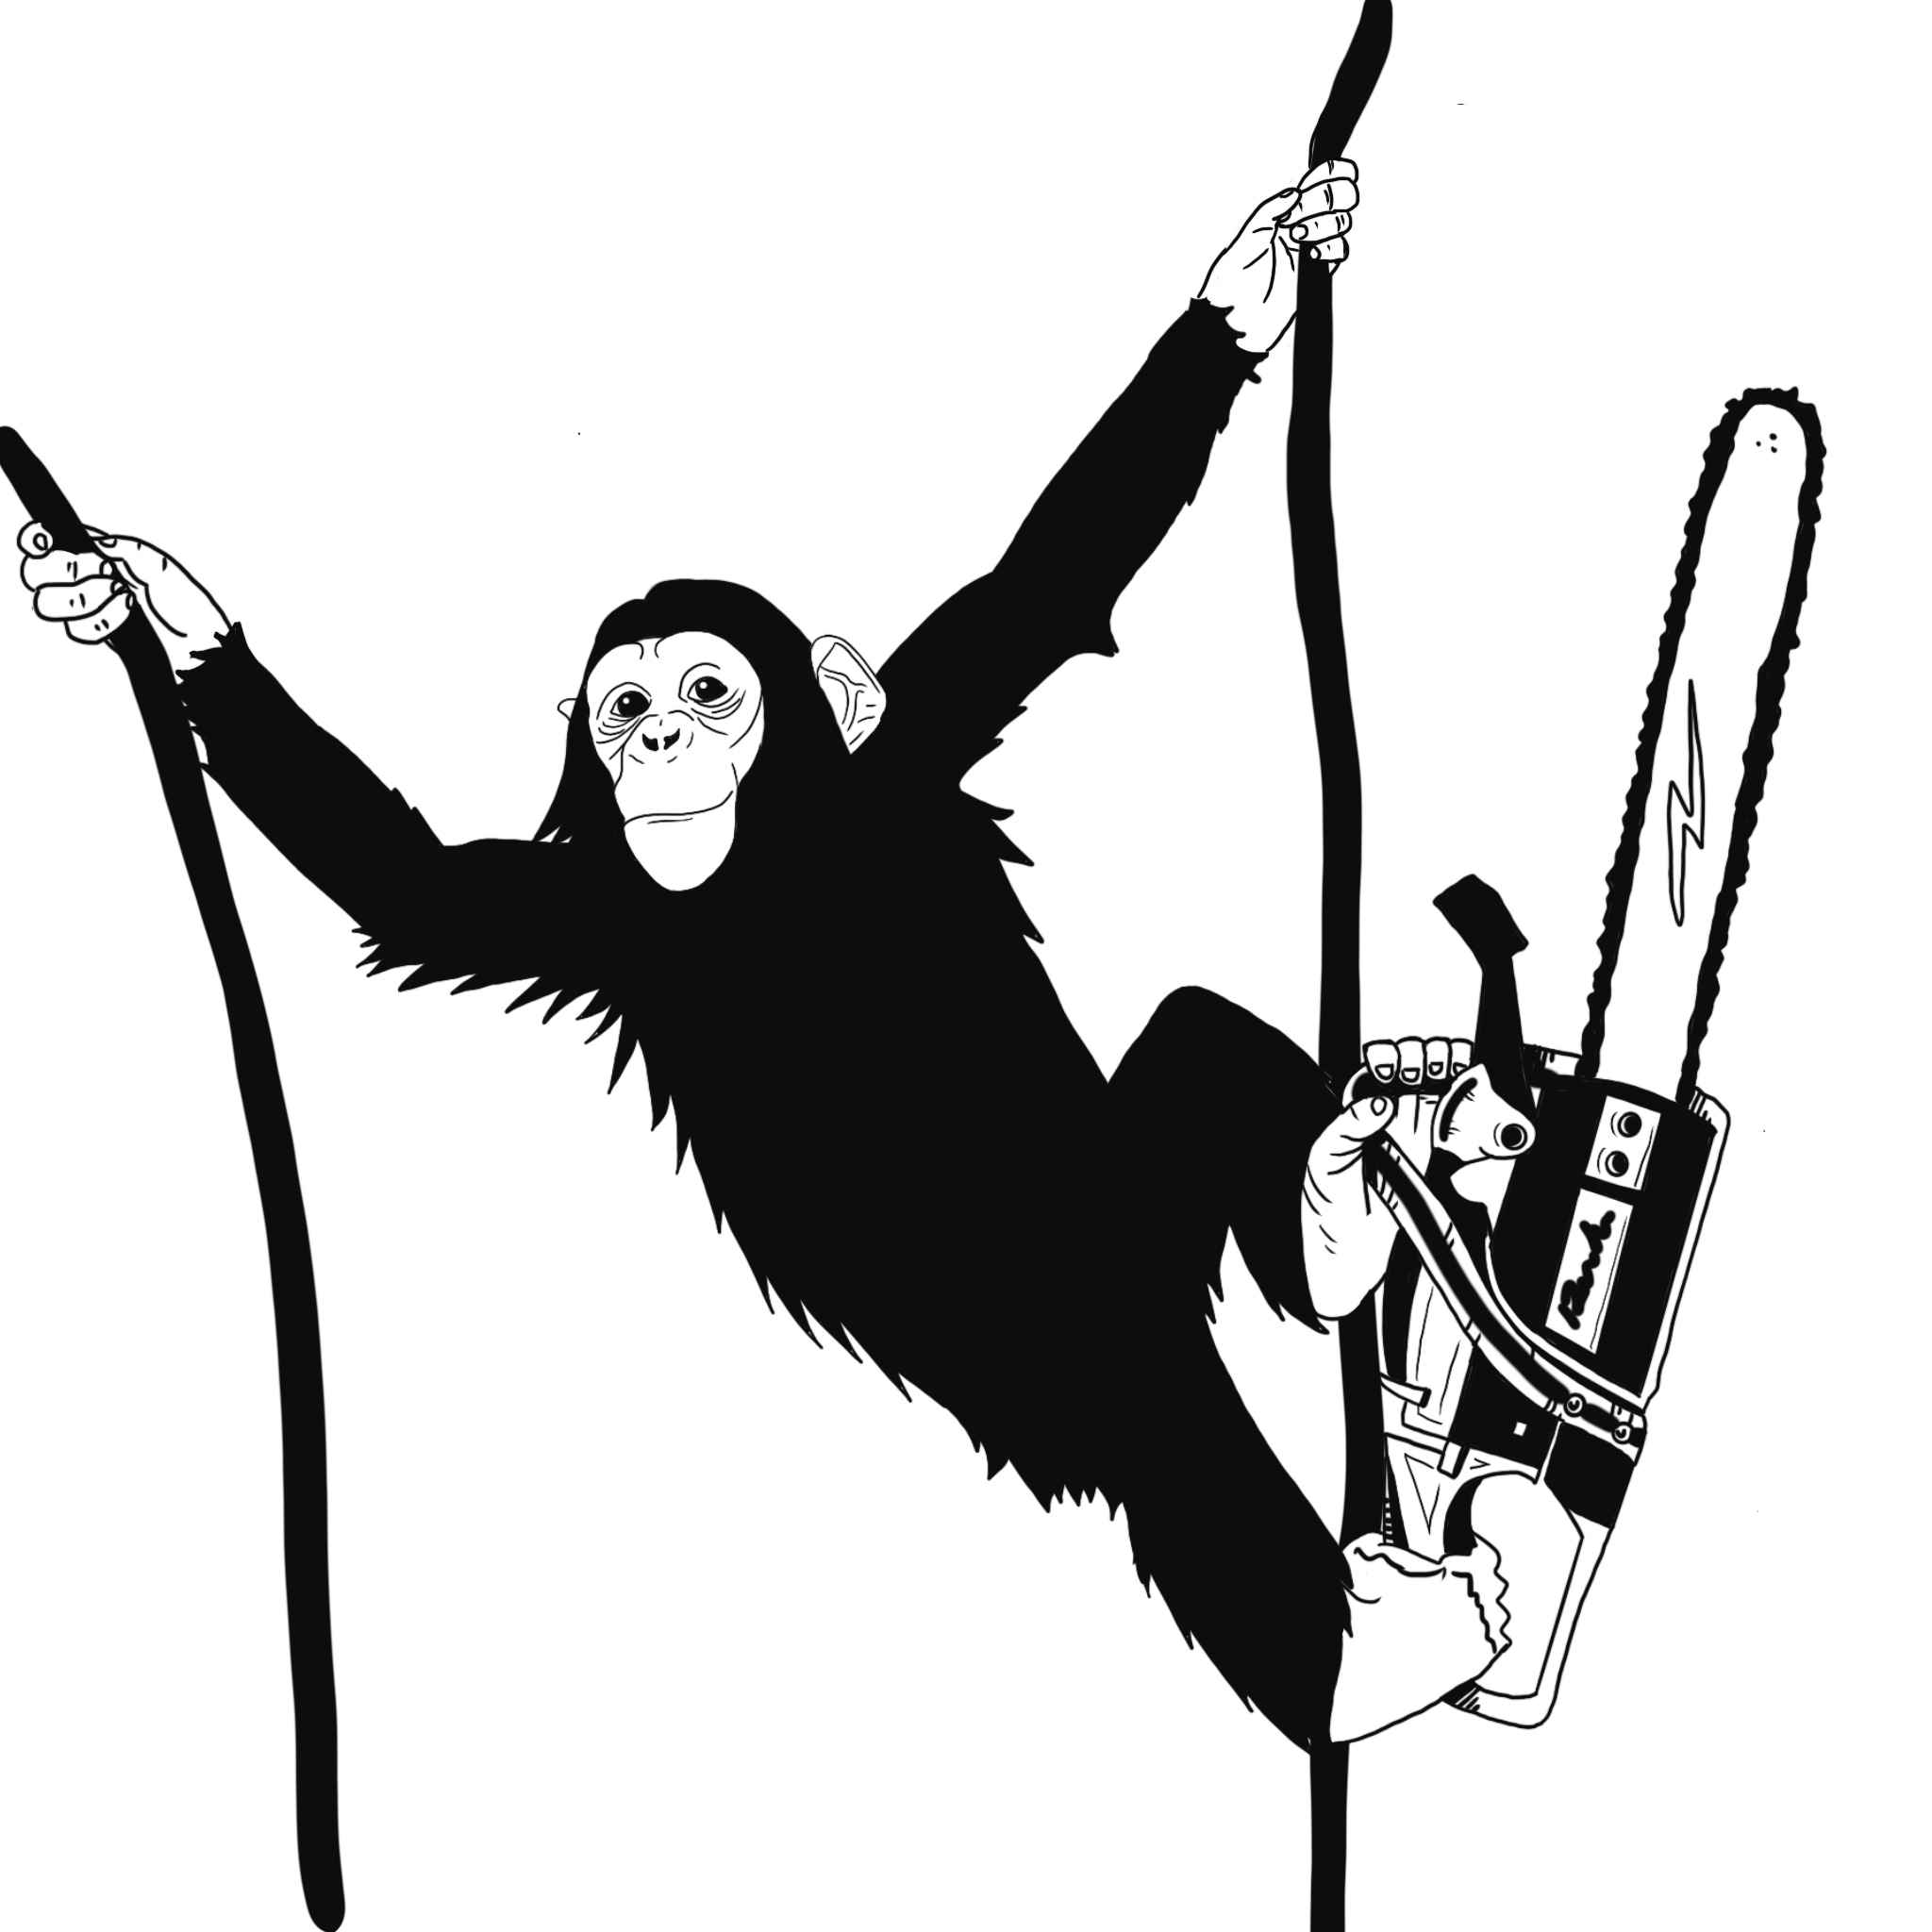
\includegraphics[width=0.35\textwidth]{../monkey.jpg} \\
    \emph{#1}
  \end{center}
}


\title{Assignment 2 \\ A Little Slice of $\pi$}
\author{
  Prof.\xspace Darrell D.\xspace E.\xspace Long \\
  CSE 13S -- Fall 2021
}
\date{Due: October $10^\text{th}$  at 11:59\,pm}

\begin{document}

\maketitle

\section{Introduction}

\epigraphwidth=0.67\textwidth
\epigraph{\emph{Dire Straits is a great band. Someone tells you they like
`Brothers in Arms' and immediately you know they're a stupid annoying}
\texttt{git}.}{---Alexei Sayle}

\noindent The aim of this first assignment will be for you to set up your
GitLab repositories and gain an understanding of how \texttt{git} works.
We will review several \texttt{git} commands that you will help you in the long
run. This document will be helpful for troubleshooting \texttt{git} issues in
the future and also includes the submission policy. You will find this quite
helpful in the future if you ever have any issues with \texttt{git} or
submitting. \emph{Ideally,} this assignment should be completed during your
discussion section.

\section{Fundamental Constants}

\epigraph{\emph{Transcendental numbers, they transcend the power of algebraic methods.}}{---Leonhard Euler}

\noindent
We live in a world (especially if you are Platonist) that is described
by and perhaps governed by mathematics and mathematical objects. Our
world is populated by numbers---fundamental constants---that we know to
exist, but which we cannot write exactly using our decimal (or any
positional) number system. We are thus presented with a pleasant
conundrum: How do we calculate these numbers that need in order to
pursue science?

There are many little things that remind us of the wonders of the
physical world in which we live. One of the most beautiful things in
mathematics, which Richard Feynman called ``our jewel,'' is
\emph{Euler's identity}:
$$
e^{i \pi} + 1 = 0
$$
which unites the most fundamental numbers in a single formula. A simple
informal proof will show you why this is so.

The tool we will use for our proof is the \emph{Taylor series} (Brook
Taylor, 1685--1731). Taylor showed that you can write most functions as
an infinite sum (there are some restrictions). This allows us to
evaluate a function $f(x)$ near a point $a$ by writing it like this:
$$
f(x) = \sum_{k=0}^\infty \frac{f^{(k)}(a)}{k!}(x-a)^k = f(a) +
\frac{f'(a)}{1!}(x-a) + \frac{f''(a)}{2!}(x-a)^2 +
\frac{f^{(3)}(a)}{3!}(x-a)^3 + \cdots
$$
where $f'$ is the \emph{first derivative}, $f''$ is the second,
$f^{(3)}$ is the third, and so forth. For example,
$$
\sin x = x - \frac{x^3}{3!} + \frac{x^5}{5!} - \frac{x^7}{7!} +
\frac{x^9}{9!} + \cdots
$$
and similarly,
$$
\cos x = 1 - \frac{x^2}{2!} + \frac{x^4}{4!} - \frac{x^6}{6!} +
\frac{x^8}{8!} + \cdots
$$
Now, notice that \emph{sine} has the odd powers of $x$, while
\emph{cosine} has the even powers of $x$. The reason for this is simple,
it is that we are using $a = 0$, and since the $\sin ' x = \cos x$ and
$\cos ' x = - \sin x$ and since $\sin 0 = 0$ and $\cos 0 = 1$ all the
trigonometric functions drop out and just leave us with powers of $x$.
We also need to look at the exponential function,
$$
e^x = \sum_{k=0}^\infty \frac{x^k}{k!} = 1 + x + \frac{x^2}{2!} +
\frac{x^3}{3!} + \frac{x^4}{4!} + \cdots
$$
If you look carefully at the Taylor series expansion of the exponential
function, you will see that it has both the even and odd powers of $x$,
but the signs are all positive, while for \emph{sine} and \emph{cosine}
half of the terms are negative.

The imaginary number $i = \sqrt{-1}$ solves the problem for us,
$$
e^{i x} = 1+i x-\frac{x^2}{2!}-\frac{i x^3}{3!}+\frac{x^4}{4!}+\frac{i
x^5}{5!}-\frac{x^6}{6!}-\frac{i x^7}{7!}+\frac{x^8}{8!}+\frac{i
x^9}{9!}-\frac{x^{10}}{10!}+\cdots
$$
and look closely at the even numbered terms. You will see that they are
the same as $\cos x$, and if you look at the odd numbered terms, you
will see that they are the same as $i \sin x$ (you simply have to factor
out the $i$). Consequently, we see that
$$
e^{i x} = \cos x + i \sin x.
$$
If you let $x = \pi$, then
$$
e^{i \pi} = \cos \pi + i \sin \pi = -1 + i \times 0 = -1.
$$
Thus, if $e^{i \pi} = -1$ then $e^{i \pi} + 1 = 0$. If you are like most
scientists, you are left with a feeling of awe.

Can we make use of this jewel to calculate a value of $\pi$? We will
start with
        $e^{i \pi} + 1  = 0$ and subtract $1$ from both sides, and we get
        $e^{i \pi}  = -1$.
        We take the square root of both sides:
        $$\sqrt{e^{i \pi}}  = \sqrt{-1}$$ and we get
        $e^\frac{i \pi}{2}  = i$.
        We take the $i^\text{th}$ root of both sides:
        $$\sqrt[i]{e^\frac{i \pi}{2}} = \sqrt[i]{i}$$ which simplifies to
        $e^\frac{\pi}{2} = \sqrt[i]{i}$.
        We are almost finished once we take the natural logarithm of both sides:
        $\log(e^\frac{\pi}{2}) = \log(\sqrt[i]{i})$ yielding
        $\frac{\pi}{2} = \log(\sqrt[i]{i})$ which simplifies to
        $\pi = 2 \log(\sqrt[i]{i})= 2\log(i^{-i})$.
So ultimately we find that $\pi$ is the logarithm of the $i^{\text{th}}$
root of an imaginary number. We may want to contemplate the words of
Benjamin Peirce (1809--1880), a professor of mathematics at Harvard, who
said ``Gentlemen, that is surely true, it is absolutely paradoxical; we
cannot understand it, and we don’t know what it means. But we have
proved it, and therefore we know it is the truth.''

\section{Calculating $e$}

\epigraphwidth=0.75\textwidth
\epigraph{\emph{Let us change our traditional attitude to the
    construction of programs. Instead of imagining that our main task is
    to instruct a computer what to do, let us concentrate rather on
    explaining to human beings what we want a computer to do.}}
    {---Donald Knuth}

\noindent
The number $e$, also known as \emph{Euler's number} (Leonhard Euler,
1707--1783), is an irrational mathematical constant approximately
equal to $2.71828$, that appears pervasively in the natural and
mathematical worlds. It is the base of the natural logarithm, it
is the limit of $\lim_{n\rightarrow\infty} (1 + \frac{1}{n})^n$
which was discovered by Jacob Bernoulli in his work on the calculation
of compound interest. And, of course, it can be expressed as the
Taylor series: $$ e=\sum_{k=0}^\infty \frac{1}{k!} =
1+\frac{1}{1}+\frac{1}{2}+\frac{1}{6}+\frac{1}{24}+\frac{1}{120}+\frac{1}{720}+\frac{1}
{5040}+\frac{1}{40320}+\frac{1}{362880}+\frac{1}{3628800}+\cdots
$$

How many terms must you compute? Fewer than you might expect, since $k!$
grows very fast. You will be determining that experimentally as part of this assignment.

\begin{figure}[bth]
\begin{centering}
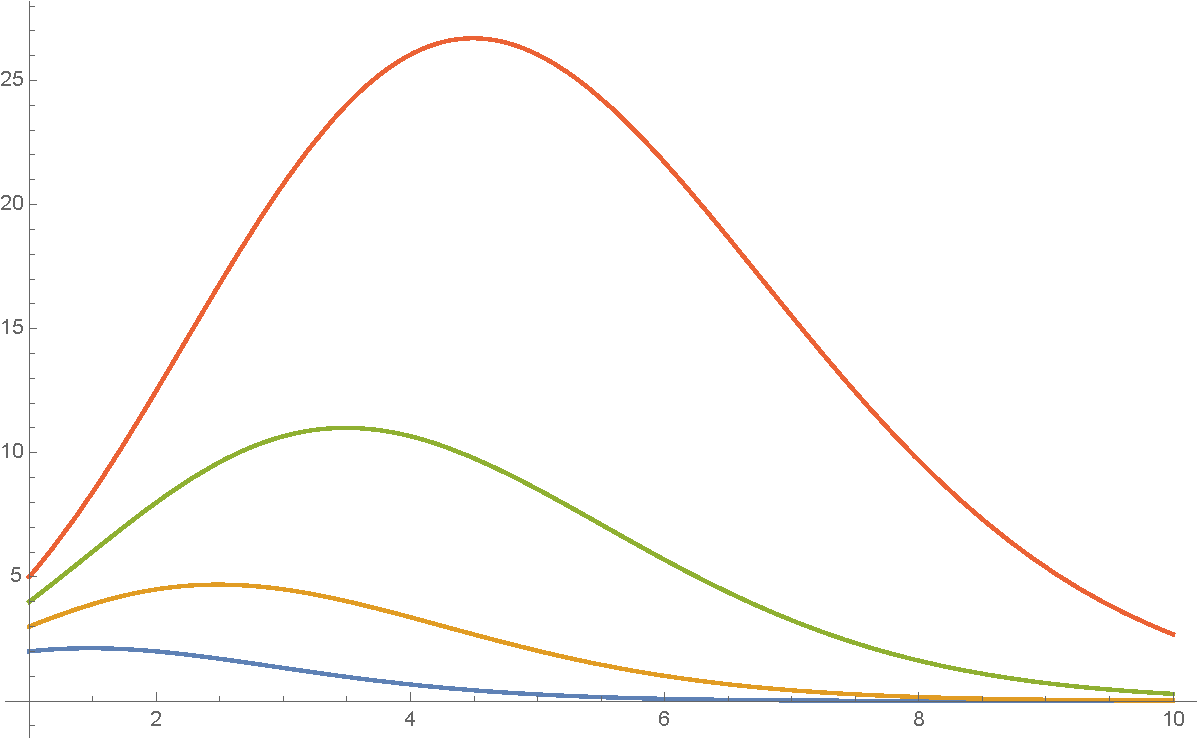
\includegraphics[width=0.75\textwidth]{images/growth.pdf}
\caption{Comparing $\dfrac{x^k}{k!}$ for $x=2,3,4,5$.}\label{growth}
\end{centering}
\end{figure}

If we are na\"ive about computing the terms of the series we can quickly
get into trouble --- the values of $k!$ get large \emph{very quickly}.
We can do better if we observe that:
$$
\frac{x^k}{k!} = \frac{x^{k-1}}{(k-1)!} \times \frac{x}{k} .
$$

At first, that looks like a recursive definition (and in fact, you could
write it that way, but it would be wasteful). As we progress through the
computation, assume that we know the previous result. We then just have
to compute the next term and multiply it by the previous term. At each
step we just need to compute $\frac{x}{k}$, starting with $k = 0!$
(remember $0! = 1$) and multiply it by the previous value and add it
into the total. It turns into a simple \texttt{for} or \texttt{while}
loop.

\section{Calculating $\pi$}

\epigraph{\emph{The best programs are written so that computing machines
    can perform them quickly and so that human beings can understand
    them clearly. A programmer is ideally an essayist who works with
    traditional aesthetic and literary forms as well as mathematical
concepts, to communicate the way that an algorithm works and to convince
a reader that the results will be correct.}}{---Donald Knuth}\noindent

Why, you might ask, do we need to calculate $\pi$? In practice, we do
not: it is available as part of the of the \texttt{<math.h>} library as
\texttt{M\_PI}, but we do need it for all manner of scientific and
engineering calculations.  The area of a circle is $\pi r^2$ and the
volume of a sphere is $\frac{4}{3} \pi r^3.$  The cosmological constant
is $$\Lambda = \frac{8 \pi G}{3 c^2} \rho.$$  Heisenberg's uncertainty
principle is given by $$\Delta x \Delta p \ge \frac{h}{4 \pi}.$$
Einstein's general relativity field equation is $$R_{\mu\nu} -
\frac{1}{2}g_{\mu\nu} +\Lambda g_{\mu\nu} = \frac{8 \pi G}{c^4}
T_{\mu\nu},$$ and so forth. No matter where you look, $\pi$ is pervasive
in the physical world.

So why do we calculate it? Well, suppose the person who typed up the
\texttt{<math.h>} file made a mistake.  Or, perhaps you need more
accuracy than is normally provided. But ultimately, most people do it
for the sheer fun of it. Computations such as finding the most digits of
$\pi$ fall into the area of experimental mathematics.

Experimental mathematics is an approach to mathematics in which
computation is used to investigate mathematical objects and identify
properties and patterns. It has been defined in a discussion by
J.\xspace Borwein, P.\xspace Borwein, R.\xspace Girgensohn and S.\xspace
Parnes as ``that branch of mathematics that concerns itself ultimately
with the codification and transmission of insights within the
mathematical community through the use of experimental (in either the
Galilean, Baconian, Aristotelian or Kantian sense) exploration of
conjectures and more informal beliefs and a careful analysis of the data
acquired in this pursuit.''

In the subsequent sections, we will present a number of functions $p$
of $n$ that are series that can be used to approximate $\pi$. In each of
these formul\ae\xspace there is a $p(n)$ where the limit
$$\lim_{n\rightarrow\infty} p(n) = \pi.$$ We know, both through
experiment (which usually comes first) and mathematical proof, that
these do result in $\pi$. The question then is: Which of these compute
it most efficiently? Efficiency in this case is measured in the
\emph{number of terms} (or factors, in the case of Wallis and Vi\`{e}te).

\subsection{The Leibniz Formula}

The Leibniz formula for $\pi$ (Gottfried Wilhelm von Leibniz, 1646--1716), given by
$$
p(n)=4 \sum _{k=0}^n \frac{(-1)^k}{2 k+1} = 4 \left ( 1 - \frac{1}{3} +
\frac{1}{5} - \frac{1}{7} + \frac{1}{9} - \cdots\right ) =
\left((-1)^n
   H_{\frac{n}{2}+\frac{1}{4}}-H_{\frac{n}{2}-\frac{1}{4}}\right)+\pi
$$
converges \emph{extremely slowly}, since the \emph{error term} involves \emph{harmonic numbers}, and consequently is not reasonable
for calculation. It is no more than the Taylor series expansion of
$\tan^{-1} x$ with $x=1$.

\begin{figure}[p]
  \centerline{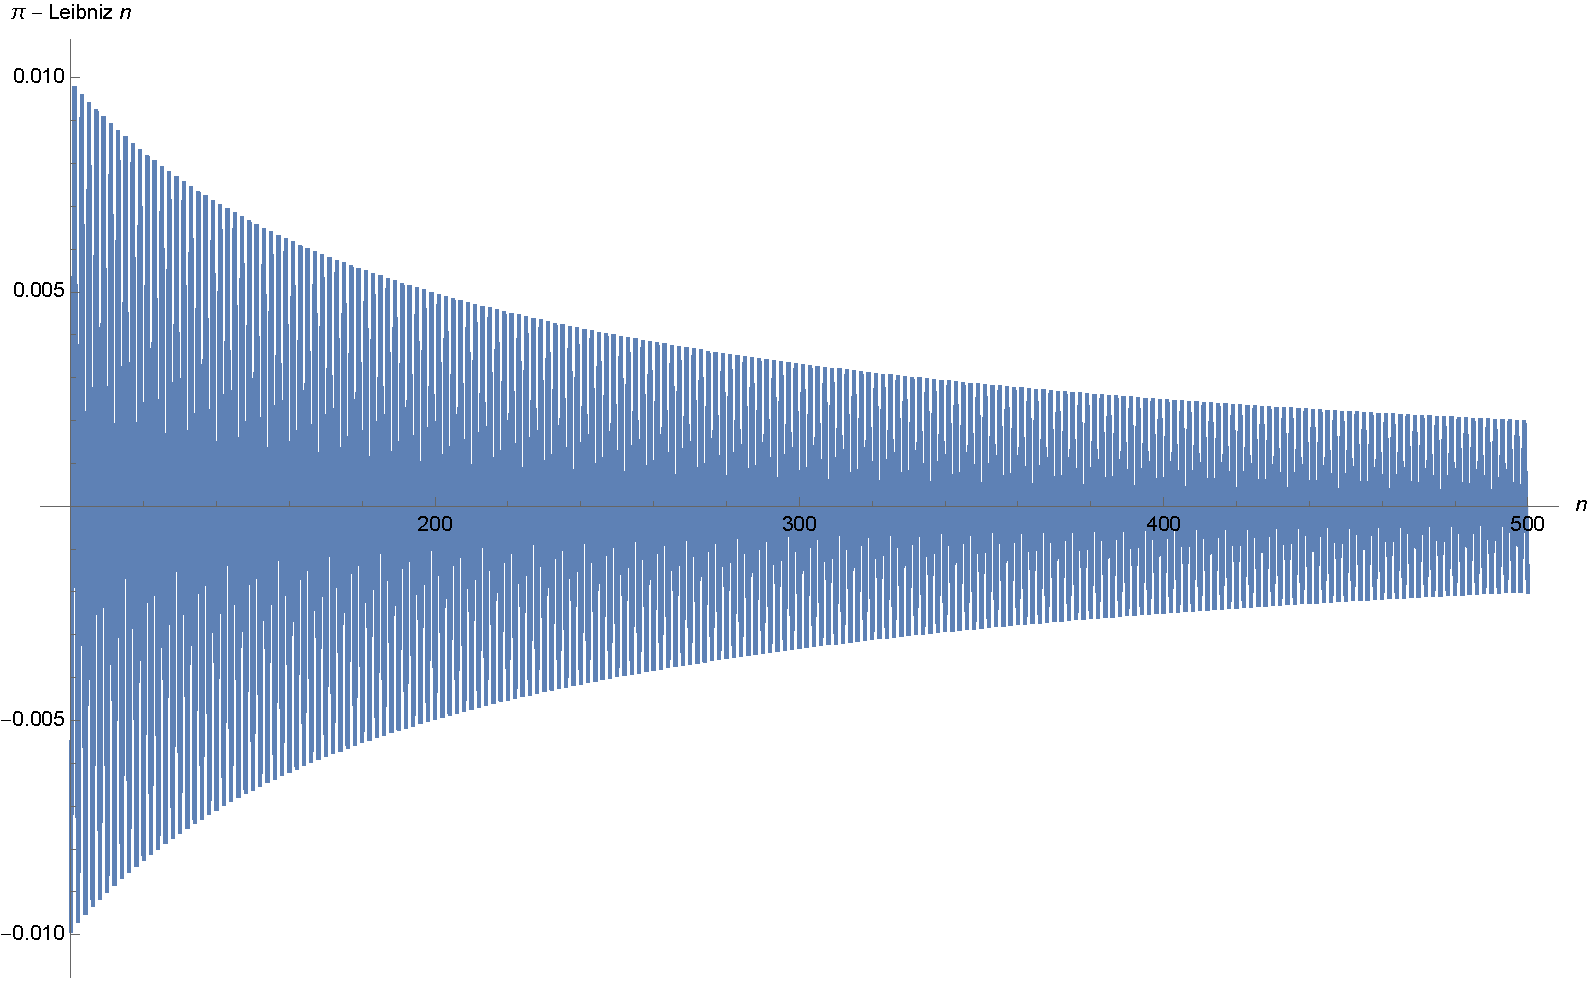
\includegraphics[width=0.75\textwidth]{figures/Leibniz.pdf}}
  \caption{Leibniz sequence $4 \sum _{k=0}^n \frac{(-1)^k}{2 k+1}$}
\end{figure}

\subsection{The Madhava Series}

The Madhava series (M\={a}dhava of Sangamagr\={a}ma, c.\xspace 1340 --
c.\xspace 1425) is also related to $\tan^{-1} x$,
$$
\sum_{k=0}^\infty \frac{(-3)^{-k}}{2 k+1} =\sqrt{3} \tan^{-1}
\frac{1}{\sqrt{3}} = \frac{\pi}{\sqrt{12}}
$$
but it gives us a more rapidly converging series, given by:
$$
p(n)=\sqrt{12} \sum _{k=0}^n \frac{(-3)^{-k}}{2 k+1} =
\sqrt{12} \left [ \frac{1}{2} 3^{-n-1} \left((-1)^n \Phi \left(-\frac{1}{3},1,n+\frac{3}{2}\right)+\pi
   3^{n+\frac{1}{2}}\right) \right ].
$$
Which leaves us with the problem of calculating $\sqrt{12}$. You may be
thinking: ``Can't I just use the library?'' The answer, of course, is
\emph{no}, you will need to compute $\sqrt{12}$ on your own.
Do you need to worry about $\Phi$? No, you just need to understand that in the limit,
the $\Phi$ term (called the \emph{Lerch transcendent})
 goes to \emph{zero} and that the remaining term
$$
\frac{\pi}{2} 3^{-n-1} 3^{n+\frac{1}{2}} = \frac{\pi}{2 \sqrt{3}} = \frac{\pi}{\sqrt{12}}.
$$

\begin{figure}[p]
  \centerline{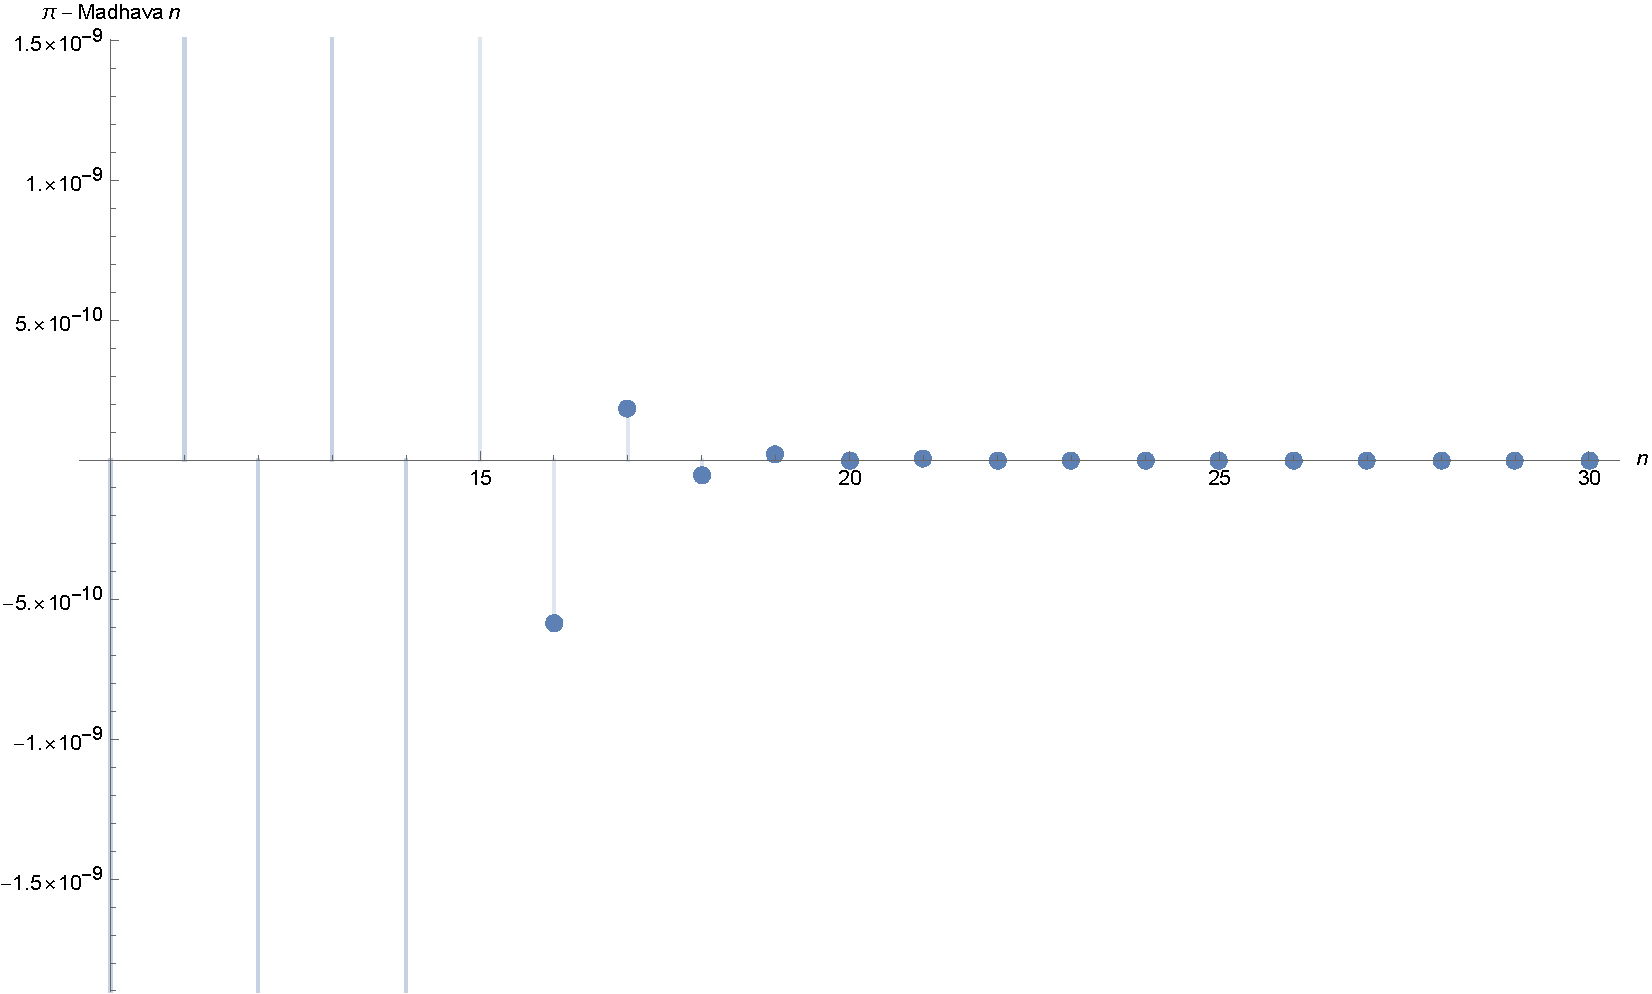
\includegraphics[width=0.75\textwidth]{figures/Madhava.pdf}}
  \caption{Madhava sequence $\sqrt{12} \sum _{k=0}^n \frac{(-3)^{-k}}{2 k+1}$}
\end{figure}

\begin{figure}[p]
  \centerline{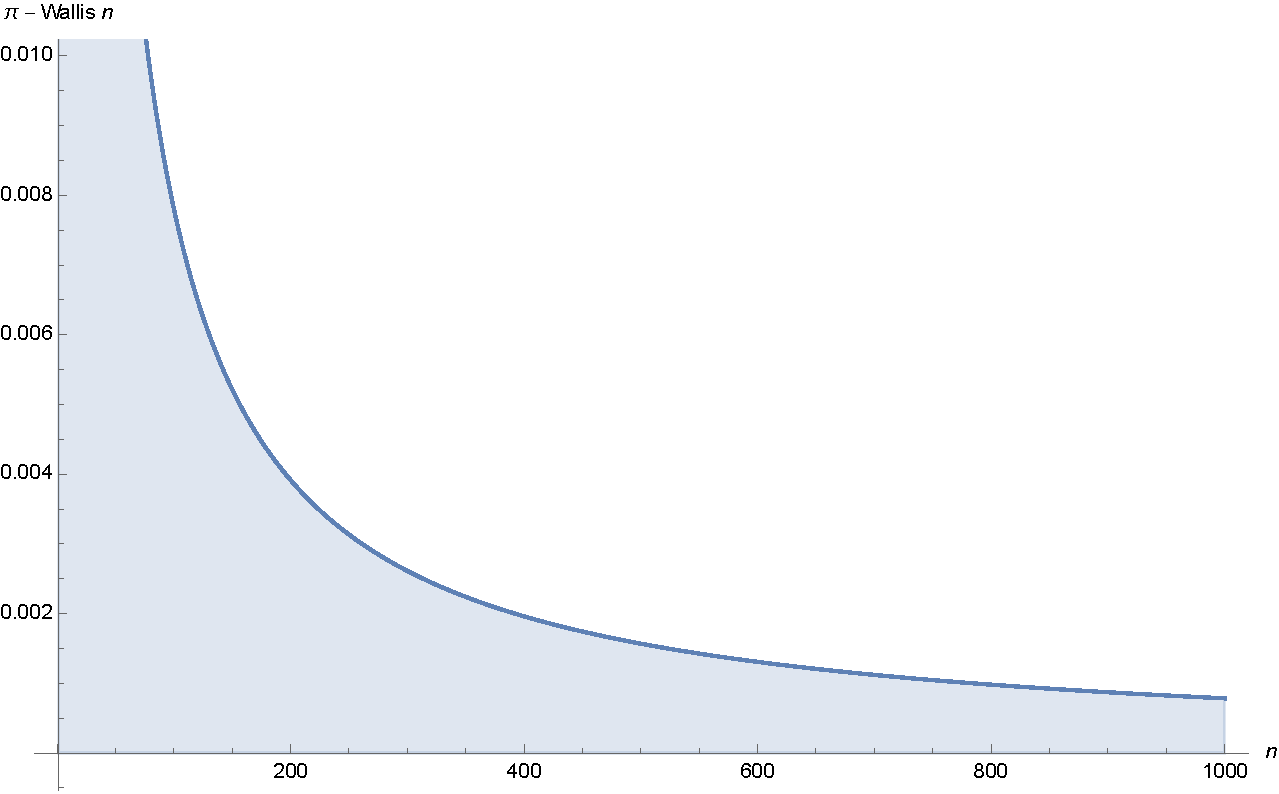
\includegraphics[width=0.75\textwidth]{figures/Wallis.pdf}}
  \caption{Wallis sequence $2 \prod _{k=1}^n \frac{4 k^2}{4 k^2-1}$}
\end{figure}

\subsection{The Wallis Series}

John Wallis (1616--1703) was an English clergyman and mathematician who
is given partial credit for the development of infinitesimal calculus.
He gave us a series that is purely multiplicative (instead of terms, we
have factors):
$$
p(n)=2 \prod _{k=1}^n \frac{4 k^2}{4 k^2-1} = \frac{\pi  \Gamma (n+1)^2}{\Gamma \left(n+\frac{1}{2}\right) \Gamma
   \left(n+\frac{3}{2}\right)}.
$$
It is easy to calculate, but how rapidly does it converge? What is this $\Gamma$ function?
Do we need to compute it?
How do we know this converges to $\pi$?
Let's factor out $\pi$, then take the limit and note that
$$
\underset{n\to \infty }{\text{lim}}\frac{\Gamma (1+n)^2}{\Gamma
   \left(\frac{1}{2}+n\right) \Gamma \left(\frac{3}{2}+n\right)} = 1.
$$
This tells us that as you compute more terms, you get closer to the true value of $\pi$.

\subsection{Euler's Solution}

The Basel problem is a problem in mathematical analysis with relevance
to number theory, first posed by Pietro Mengoli in 1650 and solved by
Leonhard Euler in 1734.  The Basel problem asks for the precise
summation of the reciprocals of the squares of the natural numbers,
\emph{i.e.}\xspace the sum of the infinite series
$$\sum_{k=1}^\infty
\frac{1}{k^2} = \frac{1}{1^2} + \frac{1}{2^2} + \frac{1}{3^2} + \cdots = H_{\infty }^{(2)},$$
which again involves harmonic numbers.
Euler's solution showed that the solution is ${\pi^2}/6$, but his method
gave us this series: $$p(n)=\sqrt{6 \sum_{k=1}^n \frac{1}{k^2}}$$ which
also requires us to calculate the square root, of this case an unknown
(until we calculate it) number.

\begin{figure}
  \centerline{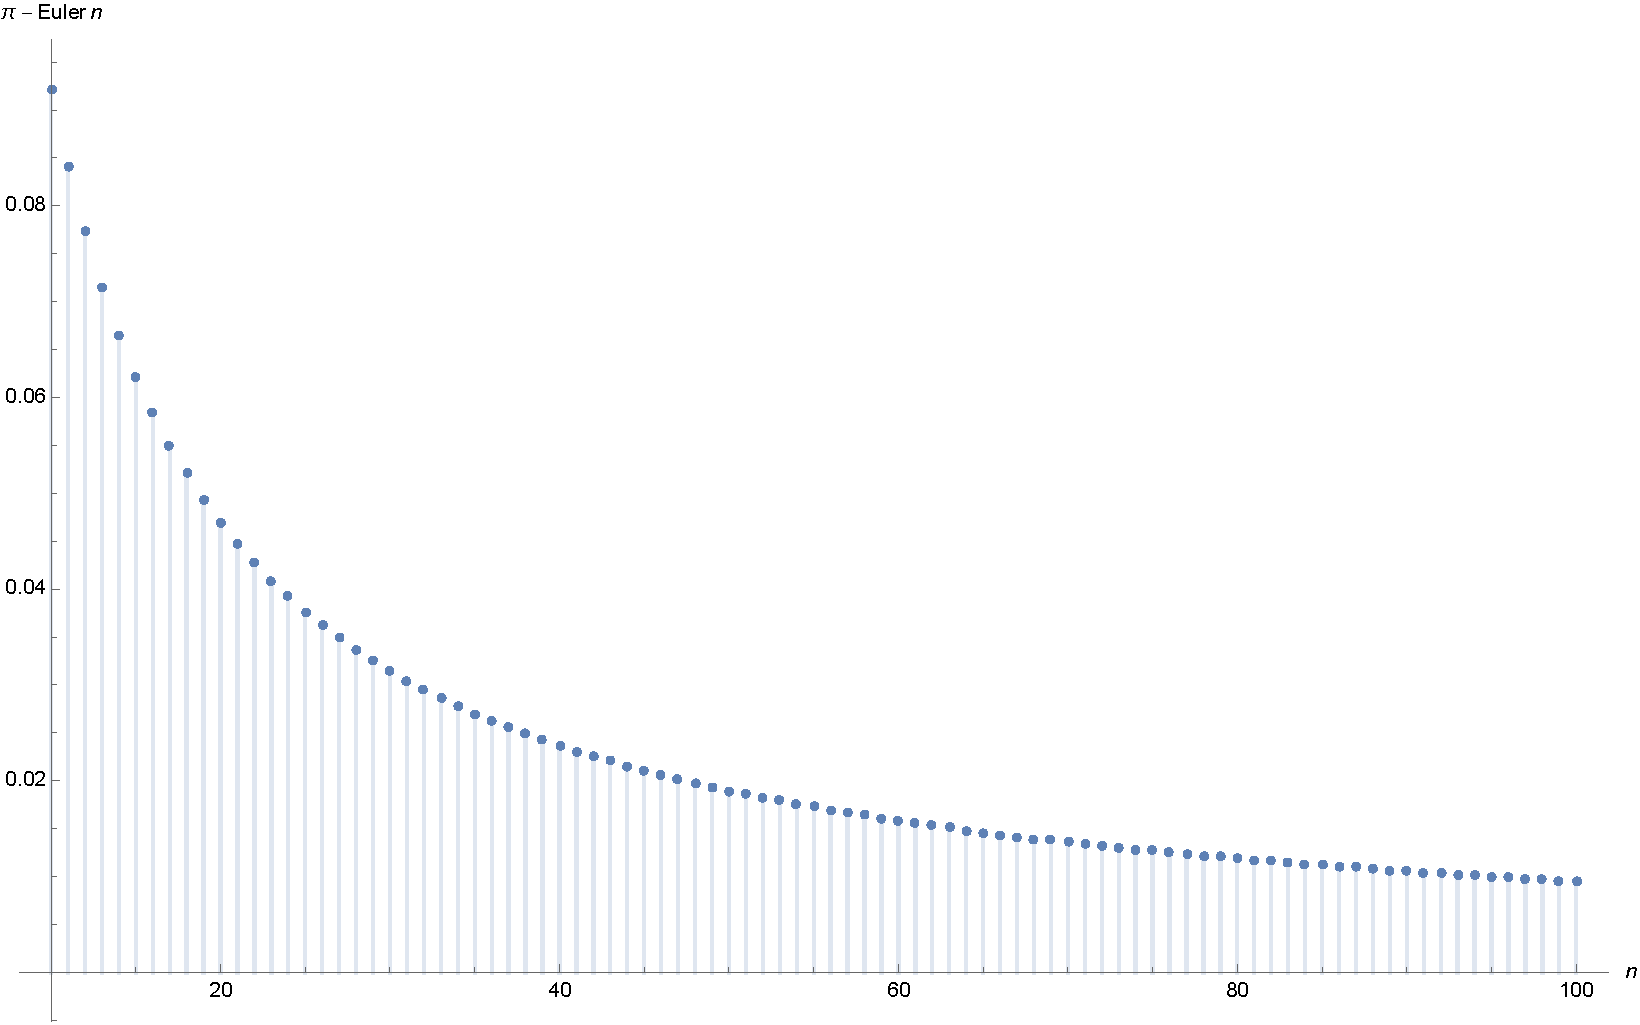
\includegraphics[width=0.75\textwidth]{figures/Euler.pdf}}
  \caption{Euler sequence $\sqrt{6 \sum _{k=1}^n \frac{1}{k^2}}$}
\end{figure}

\subsection{The Bailey-Borwein-Plouffe Formula}

The Bailey-Borwein-Plouffe formula (BBP formula) is a formula for $\pi$.
It was discovered in 1995 by Simon Plouffe and is named after the
authors of the article in which it was published, David H.\xspace
Bailey, Peter Borwein, and Plouffe. The formula that they discovered is
remarkably simple:
$$
p(n)=\sum _{k=0}^n {16^{-k}}\Biggl ( {\frac{4}{8 k+1}-\frac{2}{8
  k+4}-\frac{1}{8 k+5}-\frac{1}{8 k+6}} \Biggl ) .
$$
And if you desire to reduce it to the least number of multiplications,
you can rewrite it in \emph{Horner normal form}:
$$
p(n)=\sum _{k=0}^n {16^{-k}}\times \frac{ (k (120 k+151)+47)}{k (k (k
(512 k+1024)+712)+194)+15} .
$$

\subsection{Vi\`{e}te's Formula}

Named after Fran\c{c}ois Vi\`{e}te, Vi\`{e}te's formula is a infinite
product of nested radicals that can be used for calculations of $\pi$,
though it should be noted that methods found before this specific
formula are known to produce greater accuracy.

Vi\`{e}te's formula can be written as follows:
\[
  \frac{2}{\pi} = \frac{\sqrt{2}}{2} \times \frac{\sqrt{2 +
  \sqrt{2}}}{2} \times \frac{\sqrt{2 + \sqrt{2 + \sqrt{2}}}}{2} \cdots
\]

Or more simply,
\[
  \frac{2}{\pi} = \prod_{k=1}^{\infty} \frac{a_i}{2}
\]
where $a_1 = \sqrt{2}$ and $a_k = \sqrt{2 + a_{k-1}}$ for all $k > 1$.


\subsection{Fastest Series}

Perhaps the most interesting is the series given by Srinivasa Ramanujan
(1887--1920)
$$
\frac{1}{\pi}=\frac{2 \sqrt{2}}{9801} \sum_{k=0}^\infty \frac{(4k)!
(1101 + 26390 k)}{(k!)^4 396^{4k}}
$$
which was later extended by the Chudnovsky brothers (whose lives seem to
be centered around the calculation of $\pi$) to the series:
$$
\frac{1}{\pi} = 12 \sum_{k=0}^\infty \frac{(-1)^k (6k)! (13591409 +
545140134 k)}{(3k)! (k!)^3 640320^{3k + 3/2}} .
$$
If you can find no particular significance in the constants in
Ramanujan's formula, then perhaps we should give up any hope of
understanding the Chudnovsky's!

Ultimately, what we have learned is this: we cannot know $\pi$ exactly,
but we know relations that involve $\pi$ that we can approximate using a
series. The question then becomes: Which series converges to $\pi$ most
rapidly?

\section{The Problem of Irrationality}
\epigraph{\emph{What good your beautiful proof on the transcendence of $\pi$: Why investigate such problems, given that irrational numbers do not even exist?}}{---Leopold Kronecker}


\noindent
Hippasus of Metapontum (c.\xspace 530 -- c.\xspace 450 BC) was a
Pythagorean philosopher, usually credited with the discovery of the
\emph{irrational numbers}. According to Prof.\xspace Dimotakis, the
existence of irrational numbers was known to the Pythagoreans but
it was a closely guarded secret. Hippasus was so enthralled by the
knowledge that he went to the center of town and expounded the
discovery.  This so angered his fellow Pythagoreans, that they
drowned him in the sea.  Pappus of Alexandria merely says that the
knowledge of irrational numbers originated in the Pythagorean school,
and that the member who first divulged the secret perished by
drowning.

\begin{quote}
\emph{It is related to Hippasus that he was a Pythagorean, and that,
owing to his being the first to publish and describe the sphere
from the twelve pentagons, he perished at sea for his impiety, but
he received credit for the discovery, though really it all belonged
to \emph{him} (for in this way they refer to Pythagoras, and they
do not call him by his name).}

        \hfill{---Iamblichus the Syrian}
\end{quote}

Among irrational numbers are $\pi$ most commonly known as the ratio the
circumference of a circle to its diameter, Euler's number $e$, the
golden ratio $\varphi=\tfrac{1+\sqrt{5}}{2}$, and, as we know, the
square root of two. In fact, one can show that all square roots of
natural numbers, other than of perfect squares, are irrational.

The irrational numbers are all the real numbers (denoted by
$\mathbb{R}$) which are not rational numbers (denoted by $\mathbb{Q}$)
and those are \emph{equinumerous} with the integers (denoted by
$\mathbb{Z}$). That is, irrational numbers cannot be expressed as the
ratio of two integers. You may also be surprised to learn that
$|\mathbb{Q}| = |\mathbb{Z}|$.

When the ratio of lengths of two line segments is an irrational number,
the line segments are also described as being \emph{incommensurable},
meaning that they share no \emph{measure} in common, that is, there is
no length, no matter how short, that could be used to express the
lengths of both of the two segments as integers. Consider the triangle
$ABC$ where sides $a=1$ and $b=1$ then by the Pythagorean theorem $c^2 =
a^2 + b^2$, thus, $c = \sqrt{a^2+b^2} = \sqrt{1^2+1^2} = \sqrt{2}$. And
for this, Hippasus lost his life.

The first number to be proved irrational was the $\sqrt{2}$, probably by
our old friend Hippasus. Proofs by ancient Greeks were usually geometric
in nature, and for many, difficult to follow. Instead, let us use this
classical proof.  Suppose that $\sqrt{2}$ is rational, which means that
there exist $p$ and $q$ such that $$\sqrt{2} = \frac{p}{q}.$$ We assume
that $p$ and $q$ have no common factors, in other words, $\gcd(p,q) =1
$. If there are common factors, then we simply cancel them using the
usual method for reducing fractions. We then square both sides of the
equation resulting in $$2 = \frac{p^2}{q^2},$$ which means that $p^2 = 2
q^2$, and so $p^2$ is \emph{even}. That means that $p$ is even, and so
$p^2$ is a multiple of $4$. We can divide out $2$ and the quotient is
still even, including $q^2$, and so is $q$. If both $p$ and $q$ are
even, then they share $2$ as a common factor, contradicting our
assumption.

Like all real numbers, irrational numbers can be expressed (approximately) in positional
notation, notably as a decimal number. In the case of irrational
numbers, the decimal expansion does not terminate, nor end with a
repeating sequence. Conversely, a decimal expansion that terminates or
repeats must be a rational number. These are provable properties of
rational numbers and positional number systems, and are not used as
definitions in mathematics.

As a consequence of Georg Cantor's (1845--1918) proof that the real
numbers are uncountable and the rationals countable, it follows that
almost all real numbers are irrational. In other words, there are more
irrational numbers than there are rational numbers (in fact,
$|\mathbb{R}-\mathbb{Q}| = |\mathbb{R}|$).

In practice, this means that we can never exactly represent an
irrational number, even if we had infinite time and infinite space in
which to do so. We must instead be content with approximations, but
these must be of sufficient accuracy for us to engage in science,
engineering, and technology (and in the case of $\varphi$, art and
architecture).

Since, aside from perfect squares, all square roots are irrational, we
must have a method to approximately compute them. In our case, to
compute $\sqrt{x}$, you will use Newton's method, also called the
\emph{Newton-Raphson method}, by computing the inverse of $x^2$. It is
an iterative algorithm to approximate roots of real-valued functions,
\emph{i.e.}\xspace, solving $f(x) = 0$. Starting with an initial guess,
each iteration of Newton's method produces successively better
approximations. A \emph{Newton iterate} is defined as:
$$
x_{k+1} = x_k - \frac{f(x_k)}{f'(x_k)} .
$$
Each guess $x_{k+1}$ gives a successive improvement over the previous
guess $x_k$. In essence, we are using the \emph{slope of the line} at
the evaluation point to guide the next guess.  The function begins with
an initial guess $x_0 = 1.0$ that it uses to compute better
approximations. \texttt{sqrt()} is sufficiently calculated once the
value converges, \emph{i.e.}\xspace when the difference between
consecutive approximations is sufficiently small. In this case, $f(x) =
x^2 - y$, so you can see that $f(x)=0$ when $x = \sqrt{y}$.

\begin{pylisting}{}
def sqrt(x):
    z = 0.0
    y = 1.0
    while abs(y - z) > epsilon:
        z = y
        y = 0.5 * (z + x / z)
    return y
\end{pylisting}

% $$
% \frac{1}{32} \sqrt{\frac{1}{2} \left(2+\sqrt{2}\right) \left(2+\sqrt{2+\sqrt{2}}\right)
%    \left(2+\sqrt{2+\sqrt{2+\sqrt{2}}}\right)
%    \left(2+\sqrt{2+\sqrt{2+\sqrt{2+\sqrt{2}}}}\right)
%    \left(2+\sqrt{2+\sqrt{2+\sqrt{2+\sqrt{2+\sqrt{2}}}}}\right)}
% $$

\section{Your Task}

Your task for this assignment is to implement a small number of
mathematical functions ($e^x$ and $\sqrt{x}$), mimicking
\texttt{<math.h>}, and using them to compute the fundamental constants
$e$ and $\pi$. You will also need to write a dedicated test harness
comparing your implemented functions with that of the math library's,
then analyzing and presenting your findings in a writeup. The test
harness should be a program named \texttt{mathlib-test}. The interface
for your math library will be given in \texttt{mathlib.h}.
\textcolor{red}{You may not modify this file.} The following sections
will describe the functions that you need to write, and the files that
should contain the functions.

\textcolor{red}{You are \emph{strictly forbidden} to use any functions
from \texttt{<math.h>} in your own math library. You are also forbidden
to write a \texttt{factorial()} function.}

Each of the functions you will write must halt computation using an
$\epsilon = 10^{-14}$, which will be defined in \texttt{mathlib.h}. For
example, consider approximating the value of $e$. For sufficiently large
$k$, $|x^k| < k!$. As seen in Figure \ref{growth}, $x^k$ dominates
briefly, but is quickly overwhelmed by $k!$, making the ratio rapidly
approach zero.

\subsection{\texttt{e.c}}

This file should contain two functions: \texttt{e()} and
\texttt{e\_terms()}. The former function will approximate the value of
$e$ using the Taylor series presented in \S3 and track the number of
computed terms by means of a \texttt{static} variable local to the file.
The latter function will simply return the number of computed terms.

\subsection{\texttt{madhava.c}}

This file should contain two functions: \texttt{pi\_madhava()} and
\texttt{pi\_madhava\_terms()}. The former function will approximate the
value of $\pi$ using the Madhava series presented in \S4.2 and track the
number of computed terms with a \texttt{static} variable, exactly like
in \texttt{e.c}. The latter function will simply return the number of
computed terms.

\subsection{\texttt{euler.c}}

This file should contain two functions: \texttt{pi\_euler()} and
\texttt{pi\_euler\_terms()}. The former function will approximate the
value of $\pi$ using the formula derived from Euler's solution to the
Basel problem, as described in \S4.4. It should also track the number of
computed terms. The latter function will simply return the number of
computed terms.

\subsection{\texttt{bbp.c}}

This file should contain two functions: \texttt{pi\_bbp()} and
\texttt{pi\_bbp\_terms()}. The former function will approximate the value
of $\pi$ using the Bailey-Borwein-Plouffe formula presented in \S4.5 and
track the number of computed terms. The latter function will simply
return the number of computed terms.

\subsection{\texttt{viete.c}}

This file should contain two functions: \texttt{pi\_viete()} and
\texttt{pi\_viete\_factors()}. The former function will approximate the
value of $\pi$ using Vi\`{e}te's formula as presented in \S4.6 and track
the number of computed factors. The latter function will simply return
the number of computed factors.

\subsection{\texttt{newton.c}}

This file should contain two functions: \texttt{sqrt\_newton()} and
\texttt{sqrt\_newton\_iters()}. The former function will approximate the
the square root of the argument passed to it using the Newton-Raphson
method presented in \S5. This function should also track the number of
iterations taken, which the latter function will return.

\subsection{\texttt{mathlib-test.c}}

This file will contain the main test harness for your implemented math
library. It should support the following
command-line options:

\begin{itemize}
  \item \textbf{\texttt{-a}\,:} Runs all tests.
  \item \textbf{\texttt{-e}\,:} Runs $e$ approximation test.
  \item \textbf{\texttt{-b}\,:} Runs Bailey-Borwein-Plouffe $\pi$ approximation test.
  \item \textbf{\texttt{-m}\,:} Runs Madhava $\pi$ approximation test.
  \item \textbf{\texttt{-r}\,:} Runs Euler sequence $\pi$ approximation test.
  \item \textbf{\texttt{-v}\,:} Runs Vi\`{e}te $\pi$ approximation test.
  \item \textbf{\texttt{-n}\,:} Runs Newton-Raphson square root approximation tests.
  \item \textbf{\texttt{-s}\,:} Enable printing of statistics to see
    computed terms and factors for each tested function.
  \item \textbf{\texttt{-h}\,:} Display a help message detailing program
    usage.
\end{itemize}

The expected output for each of the $e$ or $\pi$ tests should resemble
the following:

\begin{shlisting}{}
$ ./mathlib-test -e -b -v
e() = 2.718281828459046, M_E = 2.718281828459045, diff = 0.000000000000000
pi_bbp() = 3.141592653589793, M_PI = 3.141592653589793, diff = 0.000000000000000
pi_viete() = 3.141592653589775, M_PI = 3.141592653589793, diff = 0.000000000000018
\end{shlisting}

Note that the newline should occur \emph{after} the printed difference.
You can refer to the reference program in the resources repostiroy for
the example output. With the statistics option enabled, the output
should resemble the following:

\begin{shlisting}{}
$ ./mathlib-test -e -b -v -s
e() = 2.718281828459046, M_E = 2.718281828459045, diff = 0.000000000000000
e terms = 18
pi_bbp() = 3.141592653589793, M_PI = 3.141592653589793, diff = 0.000000000000000
pi_bbp() terms = 11
pi_viete() = 3.141592653589775, M_PI = 3.141592653589793, diff = 0.000000000000018
pi_viete() terms = 23
\end{shlisting}

You will specially test your \texttt{sqrt\_newton()} function in the
range $[0,\,10)$ in steps of $0.1$. Again, you can refer to the
reference program in the resources repository for the example output.
Any \texttt{double} that is printed should use the following
\texttt{printf()} format specifier:

\begin{clisting}{}
double pi = M_PI;
printf("%16.15lf\n", pi); // Newline is included as an example.
\end{clisting}


\section{Command-line Options}
\epigraphwidth=0.6\textwidth
\epigraph{\emph{A few dud universes can really clutter up your basement.}}%
{---Neal Stephenson, \emph{In the Beginning\ldots Was the Command Line}}

\noindent
Your test harness will determine which of your implemented functions to
run through the use of \emph{command-line option}. In most \textbf{C}
programs, the \texttt{main()} function has two parameters: \texttt{int
argc} and \texttt{char **argv}. A command, such as \texttt{./exec arg1
arg2}, is split into an array of strings referred as arguments. The
parameter \texttt{argv} is this array of strings. The parameter
\texttt{argc} serves as the argument counter, which is the number of
arguments that were supplied. Try the following code, and make sure that
you understand it.

\begin{clisting}{Printing out supplied command-line arguments.}
#include <stdio.h>

int main(int argc, char **argv) {
    for (int i = 0; i < argc; i += 1) {
        printf("argv[%d] = %s\n", i, argv[i]);
    }
    return 0;
}
\end{clisting}

A command-line option is an argument, usually prefixed with a hyphen,
that modifies the behavior of a command or program. They are typically
parsed using the \texttt{getopt()} function. \textcolor{red}{Do not
attempt to parse the command-line arguments yourself.} Instead, use the
\texttt{getopt()} function. Command-line options must be defined in
order for \texttt{getopt()} to parse them. These options are defined in
a string, where each character in the string corresponds to an option
character that can be specified on the command-line. Upon running the
executable, \texttt{getopt()} should be used to scan through the
command-line arguments, checking for option characters in a loop.

\begin{clisting}{Parsing options using \texttt{getopt()}.}
#include <stdio.h>
#include <unistd.h>

#define OPTIONS "pi:"

int main(int argc, char **argv) {
    int opt = 0;
    while ((opt = getopt(argc, argv, OPTIONS)) != -1) {
        switch (opt) {
        case 'p':
            printf("-p option.\n");
            break;
        case 'i':
            printf("-i option: %s is parameter.\n", optarg);
            break;
        }
    }
    return 0;
}
\end{clisting}

This example program supports two command-line options, \texttt{-p} and
\texttt{-i}. Note that the option character \texttt{`i'} in the defined
option string \texttt{OPTIONS} has a trailing colon. The colon
signifies, when the \texttt{-i} option is enabled on the command-line,
that \texttt{getopt()} should search for a option argument following it.
An error is thrown by \texttt{getopt()} if an argument for a option, or
\emph{flag}, requiring one is not supplied.


\section{Deliverables}

You will need to turn in the following source code and header files:

\begin{enumerate}
  \item \texttt{bbp.c}: This contains the implementation of the
    Bailey-Borwein-Plouffe formula to approximate $\pi$ and the function
    to return the number of computed terms.
  \item \texttt{e.c}: This contains the implementation of the Taylor
    series to approximate Euler's number $e$ and the function to return
    the number of computed terms.
  \item \texttt{euler.c}: This contains the implementation of Euler's
    solution used to approximate $\pi$ and the function to return the
    number of computed terms.
  \item \texttt{madhava.c}: This contains the implementation of the
    Madhava series to approximate $\pi$ and the function to return the
    number of computed terms.
  \item \texttt{mathlib-test.c}: This contains the \texttt{main()}
    function which tests each of your math library functions.
  \item \texttt{mathlib.h}: This contains the interface for your math
    library.
  \item \texttt{newton.c}: This contains the implementation of the
    square root approximation using Newton's method and the function to
    return the number of computed iterations.
  \item \texttt{viete.c}: This contains the implementation of
    Vi\`{e}te's formula to approximate $\pi$ and the function to return
    the number of computed factors.
\end{enumerate}

You may have other source and header files, but \emph{do not make things
over complicated}. \textcolor{red}{Any additional source code and header
files that you may use must not use global variables.}
You will also need to turn in the following:

\begin{enumerate}
  \item \texttt{Makefile}:
    \begin{itemize}
      \item \texttt{CC = clang} must be specified.
      \item \texttt{CFLAGS = -Wall -Wextra -Werror -Wpedantic} must be specified.
      \item \texttt{make} must build the \texttt{mathlib-test}
        executable, as should \texttt{make all} and \texttt{make
        mathlib-test}.
      \item \texttt{make clean} must remove all files that are compiler
        generated.
      \item \texttt{make format} should format all your source code,
        including the header files.
    \end{itemize}
  \item \texttt{README.md}: This must use proper Markdown syntax. It
    must describe how to use your program and \texttt{Makefile}. It
    should also list and explain any command-line options that your
    program accepts. Any false positives reported by \texttt{scan-build}
    should be documented and explained here as well. Note down any known
    bugs or errors in this file as well for the graders.
  \item \texttt{DESIGN.pdf}: This document \emph{must} be a proper
    PDF\@. This design document must describe your design and design
    process for your program with enough detail such that a sufficiently
    knowledgeable programmer would be able to replicate your
    implementation. \textcolor{red}{This does not mean copying your
    entire program in verbatim}. You should instead describe how your
    program works with supporting pseudocode.
  \item \texttt{WRITEUP.pdf}: This document \emph{must} be a proper
    PDF\@. This writeup must include, at least, the following:
      \begin{itemize}
        \item Graphs displaying the difference between the values
          reported by your implemented functions and that of the math
          library's. Use a \textsc{Unix} tool --- not some website ---
          to produce these graphs. \texttt{gnuplot} is recommended.
          Attend section for examples of using \texttt{gnuplot} and
          other \textsc{Unix} tools. An example script for using
          \texttt{gnuplot} to help plot your graphs will be supplied in
          the resources repository.
        \item Analysis and explanations for any discrepancies and
          findings that you glean from your testing.
      \end{itemize}
\end{enumerate}

\section{Submission}

Refer back assignment 0 for the instructions on how to properly submit
your assignment through \texttt{git}. Remember: \emph{add},
\emph{commit}, and \emph{push}!

\textcolor{red}{Your assignment is turned in \emph{only} after you have
pushed and submitted the commit ID you want graded on Canvas. ``I
forgot to push'' and ``I forgot to submit my commit ID'' are not valid
excuses. It is \emph{highly} recommended to commit and push your changes
\emph{often}.}

\section{Supplemental Readings}

\begin{itemize}
  \item \emph{The C Programming Language} by Kernighan \& Ritchie
    \begin{itemize}
      \item Chapter 3 \S 3.4 -- 3.7
      \item Chapter 4 \S 4.1 \& 4.2 \& 4.5
      \item Chapter 7 \S 7.2
      \item Appendix B \S B4
    \end{itemize}
\end{itemize}


\monkey{If programming in \textbf{C} is like giving a monkey a chainsaw,
what does that make programming in \textbf{C++}?}

\centerline{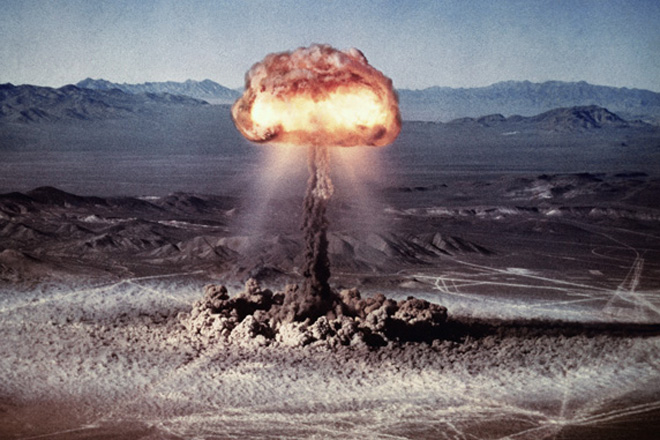
\includegraphics[width=0.75\textwidth]{./images/easy_buster_cropped.jpg}}
\end{document}
